\chapter{Understanding The Behaviour of Retweeting in Twitter}


It has been discussed that the popularity of information in Twitter can be related to the propagation characteristics of that information through Twitter's social structure. That is to say, that the more times a Tweet is retweeted by users, the more people have found the information contained within it to be interesting enough to be worth sharing.\\
It has also been shown that this retweet count metric alone cannot be an implication of the actual interestingness level of a Tweet. This is related to the notion of user influence, which directs that some tweets are naturally immediately seen by more people and thus have a higher chance of achieving a retweet as they are. Indeed, since follower count is one of the \cite{suh10} demonstrated that a user's Tweets' retweet rates increase as the user's follower count increases.

The strength of Twitter lies is in its social structure, where users can elect to follow and unfollow others as they choose. Followers of a user receive all of that user's posts in their individual (or `home') timelines. If a user has set their profile to be public, then their posts also used to appear on the public timeline, which is now deprecated but was accessible to anyone; even those without a Twitter account. As a result, people are likely to follow users who update with interesting posts; whether the follower is a big fan of the user and simply wants to know everything going on in their life, or if the follower is simply interested in the topical area of most of the friend's posts. 

Just as Twitter users will post Tweet about topics that are of interest them - possibly related to a user's work, a hobby, or a mixture of multiple areas - and these Tweets are generally posted with the idea that they will be useful or interesting for some of their followers as well as an attempt to attract more followers, retweets are generated with the same motives in mind. This means that if a Tweet is retweeted, it is not only allowed to disseminate further through the social structure, but also that a higher Tweet quality is implied.

Thus, this describes how a user's friends, who carry out retweets, effectively become filters of interesting information for that user and other followers of those friends, and the \textit{audience} of the original Tweet is significantly increased. Since retweets are always attributed to the original author then you, a Twitter user, may gain more attention by means of followers by posting \textit{interesting} Tweets, which will; 
\begin{enumerate}
\item increase the chances that users reading your Tweets will choose to follow you, and
\item increase the chances that users will decide to retweet your Tweet, thus broadcasting it to a larger audience. People viewing this \textit{retweet} then may decide to follow you. 
\end{enumerate}

Since a Tweet can be retweeted multiple times, and, as mentioned, a retweet itself can also be retweeted, the much larger the effective audience (both directly and through retweets) of a Tweet's original author has the potential to become if they choose to post interesting information. In this chapter, an understanding of the behaviours and properties of retweets is provided, along with discussions into how these are relevant in determining useful metrics for determining which retweeted information is interesting.


\section{Tweet and Retweet Properties}

\subsection{Retweet Groups}
A Tweet has various attributes associated with it, which make up the features that describe that particular Tweet. Each Tweet has a set of properties relating to its content, its author, and other metadata, such as creation time.\\
As such, a particular Tweet, $t$, can have its relevant properties declared and be defined as follows;
\[
	t = (\mathrm{text}, \mathrm{count}_R, \mathrm{author}_O, \mathrm{author}_R, \mathrm{orig})
\]

Respectively, this represents the Tweet's text, its retweet count, and the \textit{original} author of the Tweet. The final two values depend on whether $t$ is a retweet or not and represent the author of the retweet and the original Tweet respectively. Since a retweet remains a class of Tweet, then the same properties can be assigned to retweets as to Tweets, except that in the case of retweets the values $\mathrm{orig}$ and $\mathrm{author}_R$ will be non-null.

Since a Tweet can be retweeted more than once, the set of Tweets that are in the set of \textit{all} Tweets, $T$, and are retweets of $t$ is defined as;
\[
	RT(t) = \left\{ s \in T : s.\textrm{orig} = t \right\}
\]

Clearly, the retweet count of $t$ is $ t.\mathrm{count}_R = \left\vert{RT(t)}\right\vert $.

An original Tweet, $t$, along with all of the retweets of $t$, $RT(t)$, are known as the \textit{retweet group} of $t$, which is defined as $G(t)$ and is useful when discussing the audience reach of a particular Tweet. Therefore, since $t$ is also a member of this set, the size of $t$'s retweet group is; 
\[
	\left\vert{G(t)}\right\vert = t.\mathrm{count}_R + 1 
\] 
Which can have a minimum size of two - the original author and at least one retweeter. If $ r_1,...,r_n $ are the members of $RT(t)$ then the raw audience size of the group can be calculated thus (assuming $t.\textrm{count}_R \geq 1$);
\[
	\textrm{audience}(G(t)) = \textrm{followers}(t.\textrm{author}_O) + \sum\limits_{i=1}^{t.\mathrm{count}_R} \textrm{followers}(r_i.\textrm{author}_O)
\]

However, properties of Twitter dictate that this raw audience size is not an accurate calculation in most cases, as is discussed later in this chapter.


\subsection{Retweet Trees}
As a Tweet gains in popularity and attracts more and more retweets to be created from it, and since retweets themselves can also be retweeted, then this ultimately results in the generation of a retweet \textit{tree}, which represents the retweet group of a particular Tweet. This tree is formed from the \textit{users} who have retweeted the Tweet (or a retweet of the Tweet), and represents the original Tweeter and the various pathways taken by the Tweet as it is retweeted through the social graph.\\
\cite{kwak10} also uses retweet trees to assist in illustrating information dissemination in Twitter, particularly in observing the Twitter reactions to the 2009 Air France airline crash.

The tree is not a representation of the actual social ties between the tree's nodes, as users are able to retweet Tweets and retweets sent from others that they do not follow. However, as is mentioned later in this chapter, most retweeting does generally occur between directly-linked users.

The root of the tree representing every $G(t)$ is $t.\textrm{author}_O$ and, if $t$ has been retweeted, each of the other nodes are $$r_1.\textrm{author}_R, ... , r_n.\textrm{author}_R \: \forall \: 1 \leq n \leq t.\mathrm{count}_R $$\\
A similar illustrative device is used by \cite{galuba10} in describing URL \textit{cascades} in Twitter.

\begin{figure}[h]
\centering
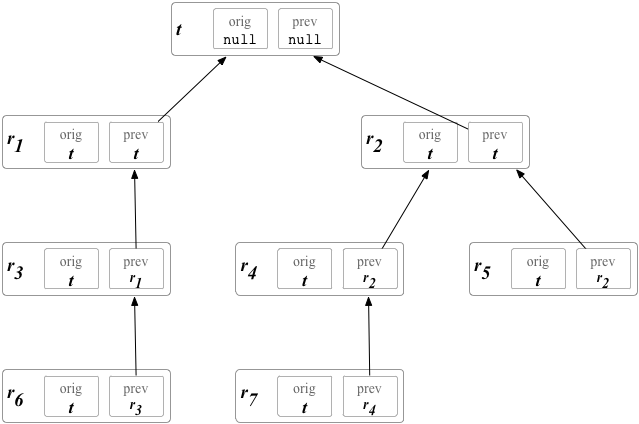
\includegraphics[scale=0.5]{3.Chapter1/Media/tree.png} 
\caption{\textit{A hypothetical retweet pathway tree.}}
\label{fig:retweet_tree}
\end{figure}

Although these retweet pathways can technically be acyclic through the use of the manual retweet method, the case of a user retweeting a Tweet more than once is very rare and a user retweeting a retweet that they are already part of the upstream chain of is even less likely to occur. The retweet button method simply does not support users retweeting a Tweet more than once.\\
As such, retweet trees are used in preference over retweet \textit{graphs} as they illustrate the temporal nature in terms of the order in which the retweets occur.


\subsection{Path-Length}
In addition to retweet groups having a size property, a retweet groups's branch's \textit{path-length} refers to the length of a particular retweet chain. In particular, it defines the number of times a Tweet is retweeted down one chain from the source user (the retweet group's tree's root) down to the final retweeter in the chain (a tree's leaf node).

Figure \ref{fig:retweet_tree} represents the users in the retweet group of a hypothetical Tweet.\\
This retweet group has a size of 11 and has 7 distinct retweet chains, the longest of which is the one traversing users 1, 3, 6 and 11.\\
The \textit{maximum} path-length of this retweet group is therefore 3, as the leaf node of this branch is three hops away from the original author at the root.

As has been mentioned previously, when a user retweets a Tweet or retweet through the manual approach, it involves pre-pending the current state of the Tweet with the text \texttt{RT @<username>:}.\\
Therefore, the Tweet with the content;\newline
\texttt{RT @user2: RT @user1: This is the body of the Tweet}\newline
was originally authored by \texttt{user1}, then retweeted by \texttt{user2}, and then finally retweeted by the author of this current retweet (the author of a Tweet or retweet's username is not credited in the body of the text).

It should be noted that this phenomenon can only be observed through retweets by the manual approach, since the button method always simply credits the original author, and not any of the internal members of the retweet group.

Although most retweets today are carried out using the button method, the manual approach still remained popular at the time the research in this chapter was carried out. This allowed for making useful observations of retweet patterns that would not be as prevalent later on.


\section{More on Information Retrieval}
A Twitter user electing to follow another user cannot predict precisely what the new friend will Tweet about in the future. The user has some \textit{expectation} of the type of information they are likely to receive based on the previous Tweets of the new friend, which is generally the only cue the user can use to base the follow decision on.

Part of the follow decision is based on the notion of relevance judgement, which is a notion discussed at more length by \cite{xu07} and is partly made up of the goal of achieving \textit{affective stimulation} through \textit{hedonic} searching as opposed to the use of \textit{epistemic} searching.

\subsection{Epistemic Search}
An epistemic information search is one that involves carrying out a search with the purpose of finding out information on a particular topic (or set of) to satisfy a \textit{desire for knowledge} \cite{xu10}, yet without an actual aim to solve any particular problem.

An example of this type of search is a `crawl' through Wikipedia, in which a searcher may start at one particular page of interest and then follow links within that page to other related pages of interest that stem away from the source topic. In this case, the search `parameter' is simply the name or title of the article the searcher wants to view.\\
As mentioned previously, a followship between users is effectively a search parameter in Twitter, since the following user has elected to follow the new friend to receive information from him/her. It is clear that this type of `searching' cannot be epistemic as the following user cannot know exactly the type of information they are going to receive.

\subsection{Hedonic Search and Affective Stimulation}
Hedonic searching is similar to epistemic searching in that it is also not carried out with the aim to solve an immediate problem, but is different in that it is done to search for fun or `affective stimulation' \cite{xu10}.

A person can be said to be affectively stimulated if they view a piece of information that has some effect on the person, such as an emotional effect, something that is of particular interest to the person, or something that is capable of provoking some further thought.

With hedonic searching, users are not aware of the information that they are going to receive prior to searching and thus cannot really predict any level of affective stimulation.\\
This aligns more with Twitter usage, since users receive information that they cannot accurately predict. Any Tweets received that do and provide interesting information convey affective stimulation to the user. This is the type of information that becomes harder to identify amongst lots of noise, yet is also the type of information a user is more likely to retweet.

\subsection{The Recognition Heuristic} 
A further metric for measuring information relevance in information retrieval is the recognition heuristic.\\
The recognition heuristic takes advantage of a person's memory and declares that if a person is able to recognise only one of two (or more) items, then he/she is more likely to judge the recosnided item to be `greater' or more important \cite{oppenheimer03} \cite{goldstein99}.

Relating this to information received on Twitter, \cite{chorley12} found that a user recognising a Tweet's author significantly increases the chance that the user will decide to read the Tweet. Since a user must read a Tweet in order to make a decision on whether, or not, to retweet it, then the recognition heuristic transiently plays a part in a user's retweet decision also.

The authors also find that information about the Tweet itself, such as its text content and its retweet count, has much more of an effect on a user's read decision than information about the author, such as the followers count or Tweet rate. This also contributes to the declaration that information interest goes beyond the features surrounding a particular user and that user influence does not dictate interestingness of information.


\section{Twitter Propagation Analysis}
Understanding information propagation in Twitter is the key to also understanding how interesting information might be detected. Whilst it is known that the retweet count of a Tweet cannot be used alone in inferring interestingness, since this is simply a level of popularity tied in with the author user's influence, it is still a factor in that users are more likely to retweet interesting information than noise.

Of particular interest is to achieve an overview of propagation behaviours in Twitter, the patterns in the properties of retweet groups, such as their sizes and penetration depth, temporal aspects of retweets and information on the social structure of Twitter itself with regards to propagation within it.

The remainder of this chapter involves an exploratory study of the retweet characteristics in Twitter to provide a further background, and which demonstrates the area's relevance towards the goal of inferring interesting information.


\section{Retweet and Retweet Group Analysis}
To assist in providing a further grounding in this area of research, a series of analyses were carried out into retweets and retweet groups. This section describes the processes and purpose of the analyses.


\subsection{Data Collection Methodology}
The analyses involve the examination of Tweets extracted from Twitter. Twitter's REST API v1 was used between 26\textsuperscript{th} January and 24\textsuperscript{th} May to collect around 26,000 Tweets, which represent a total of around 4,400 retweet groups. The complete set is made up of three subsets, the use of each individually is described later.\\
The relatively limited size of the dataset is acknowledged, yet it should be emphasised that these analyses are simply exploratory and are not used to answer or solve any specific problem.

The data collection involved a mixture of using Twitter's timelines and its search capabilities. Version 1 of the REST API supported retrieval of Tweets, 20 at a time, from the Twitter \textit{public} timeline. Historically, this timeline contained the 20 most recent Tweets published by all the authors that have non-protected Twitter accounts and used to be visible on their website's homepage\footnote{http://twitter.com} to non-logged-in users.

In particular, the public timeline endpoint was queried periodically to retrieve the current set of most recent public Tweets. From all of the retrieved Tweets, the Tweets that were retweets were filtered out and stored.\\
Retweets, as mentioned earlier, are distinguishable since they start with the characters `RT' followed by a username. It should be noted that when retrieving Tweets from Twitter's APIs that even retweets that were created using the button method begin with the same character sequence, allowing detection of these also.

Following storage, the text of the retweets were parsed in order to extract the text that the original Tweet contained. Sometimes, retweets using the manual approach are used to provide additional annotation to the Tweet. Although usually this can be distinguished by the fact that the original Tweet is inside quotation marks (`` ''), this is not true in all cases, meaning that sometimes the original text could not be reliably extracted programmatically by a machine.\\
In these cases additional queries were made to Twitter's search API in an attempt to resolve the problem, yet, failing that, the retweet was discarded.

Once the original text had been successfully extracted, this was used along with other metadata as query parameters to Twitter's search API in order to try and find the original Tweet and any other retweets of this Tweet. The search API uses approximate (or `fuzzy') string matching, but quotation marks can be used to retrieve search results based on an exact string pattern\footnote{https://dev.twitter.com/docs/using-search}.

Once the API search was complete (in some cases, with Tweets achieving many retweets, many API calls were required in order to page through results), the original Tweet could easily be identified as the only one of the set \textit{not} starting with the sequence ``RT''. This provided a retweet group comprising the original Tweet and all available retweets of this Tweet.\\
On some occasions, more than one Tweet were each identified as the original Tweet and so the entire set was discarded. This could occur, for example, if many users may Tweet exactly the same text if it comes external sources, such as a news webpage, and means that the entire set of retrieved Tweets are not likely to be part of the same retweet group.
In cases where no results were returned, the retweet was discarded and assumed an orphan retweet (perhaps as a result of a retweet of a Tweet posted by a protected Twitter account). And in cases where no original Tweet could be identified, it was sometimes possible to calculate it through cross-matching against other retweets in the retrieved retweet group, but if not they, too, were discarded.

The retweet groups were finally stored along with relevant metadata in order to carry out the studies described in the following sections.


\subsection{Exploring Retweet Group Path-Lengths}
The path-lengths of each chain in a retweet group can be calculated by identifying the users involved in retweeting down that chain; from the original author to the final retweeter. The \textit{maximum} path-length of a particular retweet group is the longest path-length observed in the group.

Identification of path-lengths can be carried out through parsing the text of a retweet, and following the citations. Although it cannot be guaranteed that all users will be properly cited in a chain, and there is no realistic method to verify this, it is felt that correct citations will be made enough times to make these cases relatively insignificant.

On average, the maximum path-length observed across the retweet groups was around 1.8, with the vast majority of retweet chains being between one and two edges in length. When one considers that many retweets are made through the button method, which removes citations of internal users in the chain and simply credits the original author, which would produce many single-length retweet chains, this average could theoretically be an underestimate.\\
\cite{kwak10}'s similar obsevations in the area also indicate a large number of groups with maximum path-lengths of one and two.

The longest observed maximum path-length was nine, which is a huge depth of penetration through the social structure since the total number of users involved in propagating the Tweet was ten. This, combined with the knowledge that social networks can represent a more tightly-knit social graph than the real world's six degrees of separation (see Introduction), shows how retweeting can have a huge impact in information spread amongst millions of people very quickly.

\begin{figure}[h]
\centering
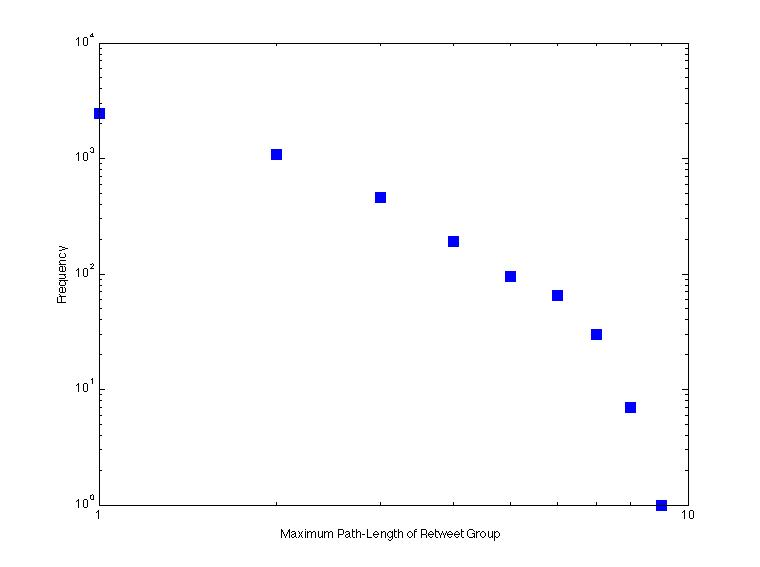
\includegraphics[scale=0.35]{3.Chapter1/Media/pathlength-distribution.jpg} 
\caption{\textit{Log/log distribution of maximum path-lengths observed across retweet groups.}}
\label{fig:pathlength-distribution}
\end{figure}

Also of interest is the relationship in terms of the social ties between different the different user members of a retweet group.\\
In cases where a retweet group's maximum path-length is precisely one, i.e. the situation where a user (or set of) has retweeted a particular Tweet only once, the retweeters at the leaves of this group's retweet tree follow the original author around 90\% of the time.

This implies, therefore, that in the remaining 10\% of cases, a retweeter has retweeted a Tweet from outside of their home timeline and has instead seen a Tweet whilst browsing through another user, who isn't a friend, timeline that the retweeter regards as sufficiently interesting.\\
This helps to demonstrate that the more followers a particular user has, the greater the chance that another user somewhere has of viewing the user's Tweets and then having the opportunity to retweet them. The fact that 90\% of retweets of a particular user are created by direct followers reinforces this further.\\
This particular property could also be due to use of the button method of retweeting, which does not cite intermediate retweeters, and thus always imply that the final retweeter directly retweeted the Tweet from the original author. However, there may, in fact, have been other retweeters in between the final retweeters and original author, each of which following the immediately upstream retweeter.

As such, this 90\% follow probability between the retweeter and source user in 1-hop retweet chains is also likely to be an underestimate.

\begin{figure}[h]
\centering
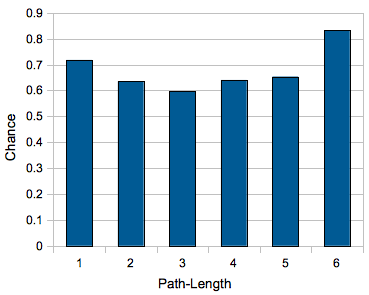
\includegraphics[scale=0.6]{3.Chapter1/Media/mentionsoriginal-pathlength.png} 
\caption{\textit{Proportion of cases where the original author is cited with varying maximum path-length of retweet group.}}
\label{fig:citation-pathlength}
\end{figure}

Further to this, in situations in which the maximum path-length of a retweet group is \textit{greater} than one, retweeting authors in the group follow the author of the original Tweet about 40\% of the time. It is clear from Figure \ref{fig:totalretweets-pathlength} that retweet groups with a longer maximum path-length tend to have a larger size themselves. This increases the likelihood that the Tweet has been able to spread both further around the original Tweet's author's community, but also the potential for the Tweet to `travel' to other communities.\\
Since users from outside the source user's community are less likely to follow the source user, this explains the reduction in the followship likelihood between further downstream retweeters in the retweet chains and the original author.


\subsection{Size of Retweet Groups}
The distribution of $|G(t)|$ across all of the original Tweets $t \in T$ collected from Twitter was found to follow a power-law type distribution, with a relatively large $p$-value of around $0.87$. \ref{fig:retweet-distribution} represents the complementary distribution function demonstrating the changing probability of a randomly generated $X$ being greater than or equal to $x$, the `current' value of $|G(t)|$, at each stage.\\
The techniques used in this analysis are adapted from the methods and code provided by \cite{clauset07}.

\begin{figure}[h]
\centering
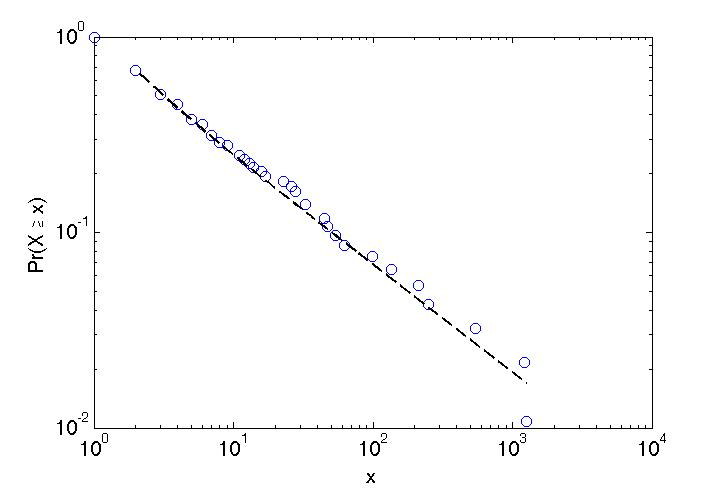
\includegraphics[scale=0.35]{3.Chapter1/Media/retweets-distribution-stats.jpg} 
\caption{\textit{Maximum likelihood power-law fit for the cumulative distribution of retweet group sizes.}}
\label{fig:retweet-distribution}
\end{figure}

The mean group size from this dataset was found to be just below six, and the largest size was 284. The smallest $|G(t)|$ were the cases in which $t.\textrm{count}_R = 1$, and which were significantly the most common occurrences.

Of interest also is the relationship between a group's size and its maximum path-length. Generally, the maximum path-length of a group, $G(t)$, increases with $|G(t)|$, indicating a mostly uniform growth in the retweet trees representing these groups - as might be expected. Thus this illustrates that as the retweet count of $t$ increases, then the longer the retweet chains in $G(t)$ are likely become. This would increase its penetrative dissemination away from the source and further facilitate its spread between communities, increasing its potential \textit{audience size}.

\begin{figure}[h]
\centering
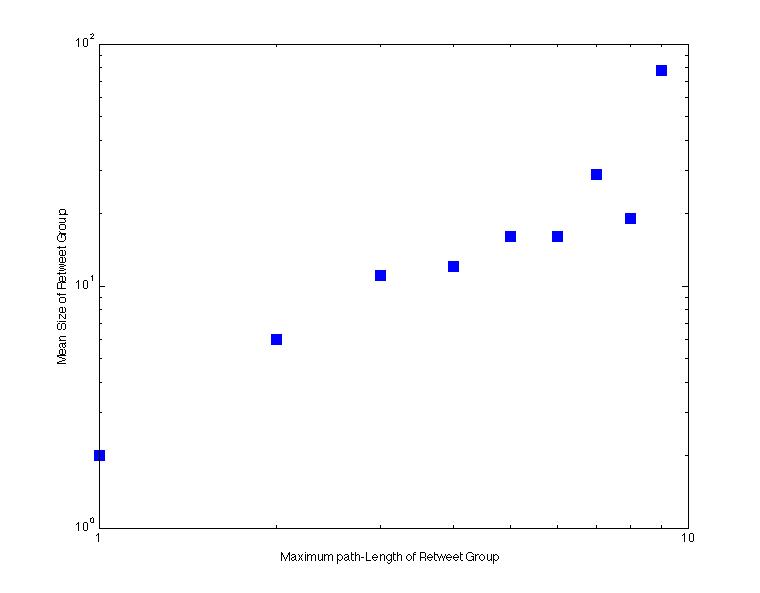
\includegraphics[scale=0.5]{3.Chapter1/Media/retweets-pathlength.jpg} 
\caption{\textit{Log/log relationship between the maximum path-length and size of a retweet group.}}
\label{fig:totalretweets-pathlength}
\end{figure}


\subsection{A Tweet's Audience - How Many Users Can be Reached?}
$G(t)$'s (immediate) audience size refers to the number of Twitter users that have received $t$, either in its original form or as a retweet, $r$, such that $r.\textrm{orig} = t$, onto their home timelines. The term `immediate' is used to signify the distinction between those users who passively receive the Tweet and those who see the Tweet whilst actively browsing through other user timelines or the public timeline.

Users in the latter group are therefore not direct followers of $t.\textrm{author}_O$ or $r.\textrm{author}_R \forall r \in RT(t)$ and thus cannot be tracked as members of $t$'s audience, which, as discussed earlier, can have its size calculated through the summation of the followers of the original author and each retweeter of $t$.

However, this audience calculation is naïve in that, particularly in the case of more tightly-knit communities, users who are authors of $t$ or $r \in RT(t)$ are likely to share a subset of each of their followers. The more dense the communities, the more followers are likely to be shared between the authors in $G(t)$ and, as such, the aforementioned audience size calculation is likely to be an overestimate in nearly all cases.\\
The following analyses of retweet group audience sizes relies on a dataset which began collecting at a later date than the general set used in this chapter, and thus the data represented in the rest of this section contains 2860 of the total 4400 groups originally collected. The longest maximum path-length of retweet groups observed in this subset was eight.

The \textit{overhead} of a group, $G(t)$, which attempts to address this problem, is related to the redundency in the audience and thus represents the number of cases in which a user receives a retweet that they have already previously received the original Tweet or retweet thereof - the number of times users receive a Tweet they've already seen. The overhead also takes into account users who might receive versions of the same Tweet many times.

This overhead was found to exist in 71\% of all observed retweet groups, further reinforcing that retweets often occur within communities containing users sharing links with other users. The \textit{proportionate} overhead is the ratio of the overhead to the \textit{distinct} audience size, which is the absolute number of users who have recieved the Tweet (or a retweet of) to their home timeline. It should be noted that the audience size does not signify the number of users who have \textit{read} the Tweet - rather the number of users who have the \textit{opportunity} to read it.

Effectively, therefore the distinct audience size of a Tweet can be found by modifying the earlier calculation:
\[
	\textrm{distinct audience}(G(t)) = \textrm{followers}(t.\textrm{author}_O) + \sum\limits_{i=1}^{t.\mathrm{count}_R} \textrm{followers}(r_i.\textrm{author}_O) - \textrm{overhead}(G(t))
\]
Where the overhead of the group is simply the magnitude of shared followers of all authors in the group.

\begin{figure}[h]
\centering
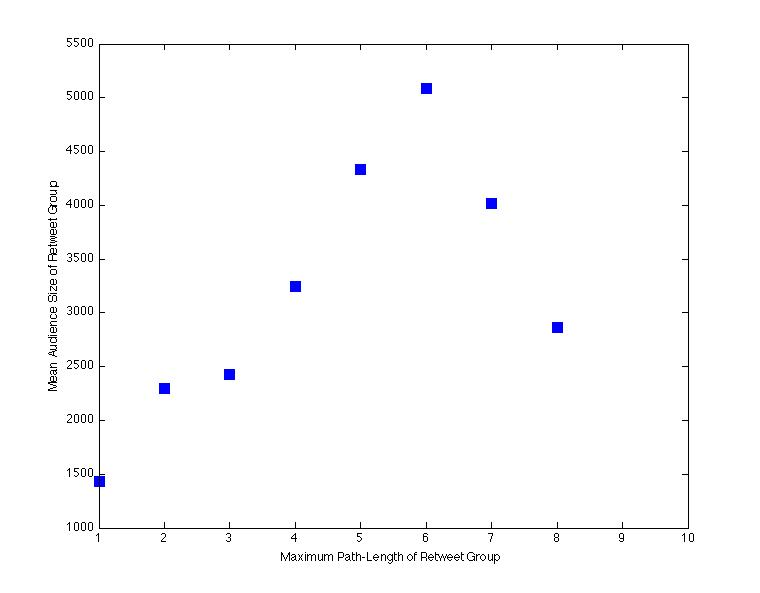
\includegraphics[scale=0.35]{3.Chapter1/Media/audience-pathlength.jpg} 
\caption{\textit{Relationship between a retweet group's distinct audience size and its longest path-length.}}
\label{fig:pathlength-audience}
\end{figure}

Figure \ref{fig:pathlength-audience} illustrates, initially, that which might be expected; that the distinct audience size of a Tweet, $t$, is mostly proportional to the maximum path length of $G(t)$. However, as the maximum path-length of retweet groups exceeds 5, then a \textit{decline} in the distinct audience size is observed. This particular behaviour has an unclear cause, but it is felt that this could be to do with a saturation in the proportionate overhead's ratio at this stage - in particular, that retweet groups attracting many retweets are circulated more within communities than outside and between communuties.\\
At this stage, the overhead becomes so large, causing this reduction in audience size. This is significant in that the distribution of the non-distict over the increasing path-lengths demonstrates, mostly, a continuous positive correlation.

Three of the largest five overheads in the set occur in retweet groups which have a maximum path-length of one. The \textit{largest} overhead was of a size over six times greater than the group's distinct audience size itself, demonstrating a massive overlap between the followers of the author of the Tweet and the authors of its retweets. Whilst the audience overhead was only found to be greater than the distinct audience size in around 3\% of observed retweet groups, it is still clear that the potential for overlap in the followers of retweet group members can be very large in more closely-knit communities - i.e. those groups whose representative trees are wide and shallow.\\
Groups having trees with longer path-lengths typically have a proportinately lower overhead, and the chance of achieving zero overhead increases as the retweet group size decreases.

The power of the retweet phenomeon in terms of how it affects the potential audience reach of a particular Tweet is discussed in further detail by the authors of \cite{kwak10}, in which they find that a retweeted Tweet of sufficient interest can reach a very large number of users even if the original author has only a few followers. The same paper more specifically mentions that the audience size of a retweeted Tweet reaches, on average, at least 1,000 users, no matter the number of followers of the original author.\\
This is also clear in the results in this thesis, in that even Tweets with a short maximum path-length can still have a relatively large audience size.


\subsection{Retweet Groups on the Social Graph}
Now that an understanding has been achieved in the behaviours and properties of retweets and retweet groups, it is important that the social ties between users in groups is studied. This will provide a grounding for the research in the following chapter, in which the social structure and its role in facilitating propagation, are discussed in more detail.

It has already been mentioned that the probability of a retweeting author following the original author in single-length retweet chains was found to be around around 90\%. However, in retweet groups with longer chains, a decrease in the likelihood of the final retweeter (the user at the bottom of the retweet tree) following the original author was observed. Indeed, on average across all retweet groups, the final retweeter follows the \textit{previous} retweeter in a particular retweet chain in around 67\% of cases.\\
The final retweeter is defined as the author of the chronologically final retweet in the group, and is not necessarily the user at the leaf node of the group's longest retweet chain.

\begin{figure}[h]
\centering
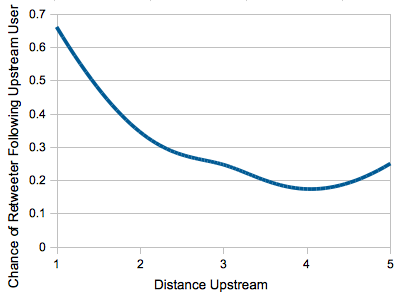
\includegraphics[scale=0.6]{3.Chapter1/Media/following-possibility.png} 
\caption{\textit{Relationship between the chance of followship between the final retweeter and original author in groups and varying maximum path-length}}
\label{fig:followingchance_pathlength}
\end{figure}

It is interesting that this value should be about 20\% lower than in single-length maximum path-length groups, and it suggests that users have a greater chance of `stumbling over' retweets found on non-friends' timelines whilst browsing through other users. Since it has been shown that with an increase in maximum path-length an increase in the audience size is also observed, then this demonstrates the increased chance of discovery of the Tweet through users searching through others' profiles.\\
In cases where the maximum path-length of $G(t)$ is equal to one, then the audience size is far smaller and thus there is a lower chance of users who aren't followers of $t.\textrm{author}_O$ or $r.\textrm{author}_R \forall r \in RT(t)$ finding the Tweet.

In addition, there is some evidence of user influence playing a role in the analyses of these data. In particular, in the 67\% of retweet groups in which the final retweeter \textit{does} follow the author of the retweet (or original Tweet) directly `upstream', the latter user has, on average, around 950 followers. Inversely, in the remaining 33\% of groups (in which the author of the final retweet does \textit{not} follow the preceding author), the preceding author has an average of 600 followers, thus implying a significant difference in the retweet potential with varying author influence levels.

This is further accentuated when one studies the follower connections of $t.\textrm{author}_O$. Whilst it was found earlier that the likelihood of a $r.\textrm{author}_R$ following $t.\textrm{author}_O$ when the maximum path-length of $G(t)$ is greater than one is around 40\%, the average follower count of $t.\textrm{author}_O$ has a four-fold increase (from about 550 to 2,000) when he/she is also followed by the final retweeter. In fact, in groups of all maximum path-lengths, $t.\textrm{author}_O$ had a consistently higher follower count when followed also by the final retweeter of $G(t)$ than when not followed.\\
This particular behaviour also helps demonstrate that a user is more likely to be retweeted when having more followers - in this case, having four times the follower count increases the correlation dramatically (40\% to 90\%). The follower count can, therefore, be directly related in this way to the discussions of user influence in \cite{cha10}, and also of users using retweeted Tweets to passively `advertise' themselves.

\begin{figure}[h]
\centering
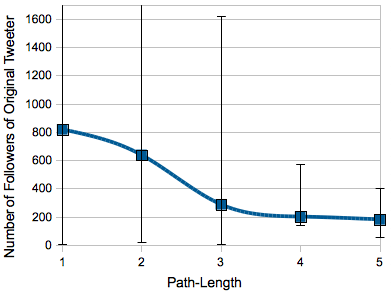
\includegraphics[scale=0.6]{3.Chapter1/Media/originalfollowers-pathlength-distribution.png} 
\caption{\textit{Relationship between number of followers (and respective distribution) of the original tweeter as the path-length increases}}
\label{fig:originalfollowers-pathlength}
\end{figure}

Strangely, it was found that $t.\textrm{author}_O$'s follower count actually diminishes with increasing maximum path-length of $G(t)$, indicating further penetrative depth of propagation when the original author has \textit{fewer} followers. The collected retweet groups that contained longer retweet chains often also contained retweet chains that were much shorter. For example, a group containing chains with path-lengths of five, or more, are also likely to contain many more chains with path-lengths of one and two (as is implied in the distribution in Figure \ref{fig:pathlength-distribution}).\\
There are, therefore, various possible explanations for this property, including the argument that users with many followers are generally likely to be part of a large community of users, from which retweets are not transmitted. Users that are part of several communities, and are therefore less involved with any given one, may find that their Tweets have the potential to be retweeted a further distance.

Additionally, and more interestingly, it is possible that users possess some awareness of their local networks and the users within them. A user, who is part of a large community with lots of obvious follower overlaps occurring between the members, may decide \textit{not} to retweet a particular Tweet if he/she feels that many of their own followers may have already seen the Tweet due to them also having a high chance of following the original author.

A final analysis on the social ties between users in retweet chains is carried out on the followship pattern of authors throughout the chain. Let $h$ be the number of hops (or edges in the retweet tree) between two users in a retweet chain. It was illustrated in earlier sections that, when $h = 1$, the likelihood of the later retweeting author following the upstream author is around 67\%.\\
However, as $h$ is increased, then the followship likelihood mostly consistently decreases (see Figure \ref{fig:following-possibility}, as might be expected. This illustrates how longer retweet chains do indeed increase both the likelihood of the Tweet reaching further through the social structure and the chance of achieving a smaller proportionate overhead.

Further to this, of the 67\% of retweeters who \textit{do} follow an upstream author at $h = 1$, only 19\% follow also the upstream author at $h = 2$. In these cases, the latter has an observed average of around 3,000 followers.\\
In the 81\% of cases when the user at $h = 2$ \textit{isn't} also followed, then the upstream author has a much lower average follower count of about 520.

\begin{figure}[h]
\centering
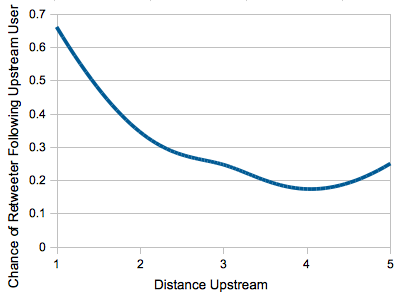
\includegraphics[scale=0.55]{3.Chapter1/Media/following-possibility.png} 
\caption{\textit{Proportion of final retweeters following upstream users at varying distances along the chain.}}
\label{fig:following-possibility}
\end{figure}

It is, therefore, sensible to assume from these analyses that Tweets are forwarded between groups of less-connected users, highlighting the notions of social network awareness and of community-hopping. If retweets were usually circulated around more closely-knit communities of users, then the followship likelihoods would be generally greater, more uniform, and consistent throughout the retweet chain. Users would have as much of a chance of following their immediate upstream neighbour author in the retweet chain as they would a further upstream author.

As mentioned near the start of this chapter, the author of the original Tweet should be cited by the \texttt{RT @<username>} sequence observed \textit{closest} to the retweet body, where \texttt{<username>} is the username of the author user. Rather than specifically looking for the author's Tweet appearing in this location, Tweets were examined to check for the existence of the author's username being mentioned \textit{anywhere} in the Tweet content, and was found to exist in about 68\% of Tweets.\\
This frequency did not vary with any consistent correlation upon changes to the maximum path-length or retweet group size, and so it is assumed that users do feel the need to credit the original author more so than not. 

 
\subsection{The Temporal Properties of Retweets}
The final set of analyses in this chapter relate to time's influence on retweet propagation. This facilitates insights into how quickly information can spread and, when combined with the knowledge of the social structure and audience, how this can relate to the rate of information dissemination and consumption.

\begin{figure}[h]
\centering
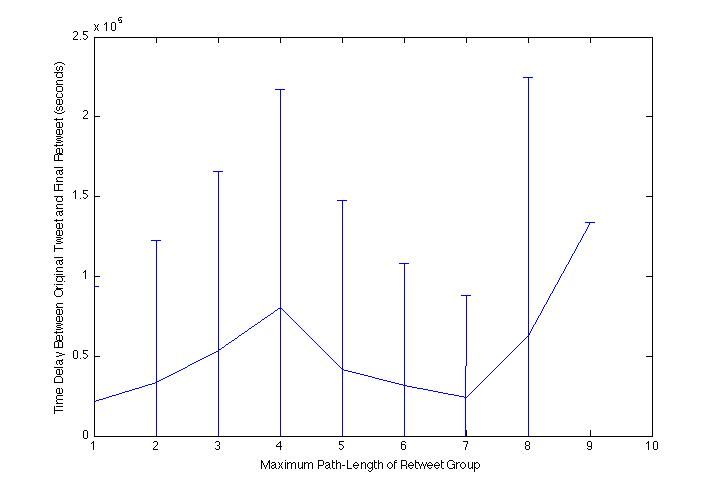
\includegraphics[scale=0.35]{3.Chapter1/Media/pathlength-timedelay.jpg} 
\caption{\textit{Average time (in seconds) between first post and final retweet of a retweet group varying with the group's maximum path-length}}
\label{fig:timedelay-pathlength}
\end{figure}

A general observation is that the elapsement of time between the original Tweet and the final retweet of retweet groups of varying maximum path-lengths increases with path-length, indicating that if there are more hops for a Tweet to travel down between users then it takes longer to do so. However, this correlation is only really applicable for shorter retweet chains and, particularly in cases where the maximum path-length is five and above, this pattern is not consistent.\\
The groups with shorter maximum path-lengths more uniformly increase in temporal elapsement with increases in maximum path-length in a linear fashion roughly proportional to $ v=\frac{s}{t} $, where the distance, \textit{s}, is the hypothetical distance given by the number of hops between users, thus indicating that the speed, $v$, of propagation remains relatively constant. 

Despite this, there are conflicting arguments for patterns observed in retweet propagation speed, which rely on various different factors.\\
As mentioned, the time taken for a Tweet to reach a specific path-length could be a function of the path-length itself, where as the path-length increases, then so does the time taken for the Tweet to be retweeted to the end of the chain.\\
Inversely, Tweets that are especially popular, possibly as a result of being particularly topical (such as in the disaster cases mentioned in the Introduction), may be retweeted more quickly by users so that the information is spread more quickly. In these cases, retweet groups with longer retweet chains may complete their trees more quickly than those groups with much shallower retweet trees.\\
Similarly, user influence could play a role in dissemination speed; if a Tweet is retweeted by a user with many followers, then there is an increased likelihood of propagation through this user. Whilst this could, in addition the previous argument, cause longer retweet trees to be completed more quickly than groups with shorter trees, it could also facilitate `faster branches', in which particular long branches grow more quickly than shorter ones in the same retweet tree if the other branches consist of less-influential users.

There is not enough evidence provided in this analysis to make any inferences towards a ganeric pattern of retweet group growth speed, and it is believed that this growth is governed by many more factors than the Tweet itself or the social structure alone. As such, there is no predefined rule for predicting the spread of dissemination in this way, since the retweet path is an unknown feature.

The temporality of retweets has been the focus of some researchers, including the authors of \cite{kwak10}, who also used retweet trees as an illustration of the propagation pattern produced by Tweets. They found that, generally, half of all retweet action on a Tweet occurs \textit{within an hour} of the Tweet being posted, and that by the end of the first day, 75\% of all retweets of the Tweet will have happened.\\
The authors also conducted an analysis on the elapsed time of a Tweet's travel between hops as it is retweeted. Although they observe a flatter time elapsement initially, indicating that Tweets travelling over the first few hops are retweeted almost concurrently, they also found there to be a general incline in time elapsement over the shorter path-lengths. After this point, as seen and discussed in the analysis earlier, the elapsement becomes more `noisy'. 

An interesting notion that is not directly addressed in this thesis is that the time a particular Tweet is authored may have some effect on its propagation speed. Just as `prime-time' television achieves higher audience ratings as it is at a time of the day when many people are at home and relaxing, Twitter may also have a time window in which its users are more active. For example, if a user posts a Tweet at a time when many of his/her followers are asleep, then the immediate audience size of the Tweet can be significantly reduced.\\
If there are fewer initial users viewing the Tweet, then the likelihood of retweet, as a function of this, is also reduced. Although this could have an effect on the perceived popularity of the Tweet, since, by definition, there are fewer active users on Twitter at this time, then the number of Tweets sent during this period will be much smaller. We therefore do not take this factor into account during our experimentation in later chapters.


\section{Summary}
In this chapter, a set of initial exploratory analyses have been undertaken into the behaviours of retweeting in Twitter, the properties of retweet groups, the relationships between the propagation graph and the social graph, and briefly into the affects of time on Tweet dissemination.

The analyses were found to support and complement the findings of other research in the area, including the notions of message cascading \cite{galuba10} and the ties of this to the interconnection of users on the social graph through communities \cite{java07}.\\
Trees representing the retweet groups were found to grow in a variety of ways, from trees illustrating long retweet chains, indicating a high level of inter-community dissemination, to shorter and wider trees, in which propagation can still be widespread but not as likely to reach other communities.

User influence, in terms of an author's follower count, was observed as being an important factor in facilitating information, implying that popular users also produce popular information, since these users are more likely to achieve more retweets.

These inferences have helped to describe the multi-dimensional principles of retweet groups in terms of the features governing their spread over the social graph, and the quickness with which many users can be exposed to a Tweet through the act of retweeting. Although it is important to have an understanding of user psychology, and the thought processes behind the retweet decision, of most interest in this chapter is the analysis of the social structure.


\section{Taking the Investigative Research Further}
Twitter's social structure has been found to have a large effect on Tweet propagation, since it combines the features observed around user influence (in the naïve form of a user's follower count) with that of communities and sub-graphs of dense and sparse user interconnections.

In the following chapter, interests are focused on the topiological structure of user followships by investigating further into the flow of information between users as they are arranged in different ways in order to develop a method to infer information interestingness taking into account these information flow properties and user influence. It is clear that different Tweets can have a different level of \textit{quality} in that Tweets that are retweeted have a greater chance of being interesting, but does the way in which the social structure of users is formed also have a quality in terms of facilitating retweeting?

%\begin{mydefinition}
% The \textbf{broadcast front}, denoted by $B_v(t)$, of token $\tau_v$ at timestep $t$ is the set of nodes that received $\tau_v$ in timestep $t$ but did not have it in timestep $t-1$.
%\end{mydefinition}

